Tritium is the only radioactive isotope of hydrogen present in the environment. It was for the first time produced in $1934$ from neutron capture of deuterium by Ernest Rutherford, Mark Oliphant and Paul Harteck \cite{TritiumDiscovery} and it was first time isolated in 1939 by Luis Walter Alvarez and Robert Cornog \cite{TritiumIsolate}, who checked that tritium is a radiactive element. 

Tritium is naturally produced in the environment through the interaction of cosmics rays and gaseous elements of the upper atmosphere like nitrogen ($\ce{^{14}N}(\ce{n},\ce{^{3}H})\ce{^{12}C}$) \cite{TritiumHandling} and oxigen ($\ce{^{16}O}(\ce{n},\ce{^{3}H})\ce{^{14}N}$) \cite{OxigenTritium}. Around 99\% of cosmogenic tritium forms water (\ce{HTO}) and reaches the Earth's surface as rain with an estimated produccion rate of $4\cdot 10^6 ~\curie/$yr ($1.48 \cdot 10^8 ~\giga\becquerel/$yr), producing a tritium concentration of $0.6-1.2~\becquerel/\liter$ in precipitation \cite{CommonEmissionTritium, TritiumHandling}. 

Tritium can be produced artificially in the environment from different anthropogenic sources \cite{CommonEmissionTritium, TritiumHandling}. There is a large amount of tritium which was produced in military nuclear test explosions between 1945 and 1975, with an estimated total production of $8 \cdot 10^9~\curie$ ($2.96 \cdot 10^{11}~\giga\becquerel$) and a part of which remains to the date. In these nuclear explosions, tritium was produced mainly from the nuclear reactions $\ce{^{14}N}(\ce{n},\ce{^{3}H})\ce{^{12}C}$ and $\ce{^{2}H}(\ce{n},\gamma)\ce{^{3}H}$. Tritium can also be  produced by commercial producers of radioluminiscent and neutron generator devices ($1 \cdot 10^6~\curie/$yr), nuclear power and defense industries (around $2 \cdot 10^6~\curie/$yr) and several research facilities and nuclear reactor for energy production ($2 \cdot 10^6 \curie/\giga\watt$yr), through the production cross sections shown in Table \ref{tab:NuclearReactionsTritiumProduction}: 

\begin{table}[htbp]
\begin{center}
\begin{tabular}{|c|c|c|c|}
\hline
Source & Origin & Nuclear reaction & Cross section ($\barn$)\\
\hline \hline \hline
$\ce{^{2}_{1}H}$ & Water coolant & $\ce{^{2}_{1}H}(\ce{n},\gamma)\ce{^{3}_{1}H}$ & $5.2 \cdot{} 10^{-4}$ \\ \hline
$\ce{^{3}_{2}He}$ & Helium coolant & $\ce{^{3}_{2}He}(\ce{n},\ce{p})\ce{^{3}_{1}H}$ & $5330$ \\ \hline
$\ce{^{6}_{3}Li}$ & Moderator & $\ce{^{6}_{3}Li}(\ce{n},\alpha)\ce{^{3}_{1}H}$ & $940$ \\ \hline
$\ce{^{10}_{5}B}$ & \parbox{8em}{\centering Moderator,\\ control rods} & $\ce{^{10}_{5}B}(\ce{n},2\alpha)\ce{^{3}_{1}H}$ & $3835$ \\ 
\hline
\end{tabular}
\caption{Most common nuclear reactions of artificial tritium production~\cite{CommonEmissionTritium}}
\label{tab:NuclearReactionsTritiumProduction}
\end{center}
\end{table}

%\begin{equation}
%\ce{^{2}_{1}H}(\ce{n},\gamma)\ce{^{3}_{1}H} \qquad \sigma= 5.2 \cdot{} 10^{-4}~\barn  ~~~\cite{CommonEmissionTritium}
%\label{eq:capneuH2}
%\end{equation}

%\begin{equation}
%\ce{^{3}_{2}He}(\ce{n},\ce{p})\ce{^{3}_{1}H} \qquad \sigma= 5330~\barn ~~~\cite{CommonEmissionTritium}
%\label{eq:capneuHe3}
%\end{equation}

%\begin{equation}
%\ce{^{6}_{3}Li}(\ce{n},\alpha)\ce{^{3}_{1}H} \qquad \sigma= 940~\barn ~~~\cite{CommonEmissionTritium}
%\label{eq:capneuLi6}
%\end{equation}

%%\begin{equation}
%%\ce{^{7}_{3}Li}(\ce{n},\alpha)\ce{^{3}_{1}He} + \ce{n} ~~~\cite{CommonEmissionTritium}
%%\label{capneuLi7}
%%\end{equation}

%\begin{equation}
%\ce{^{10}_{5}B}(\ce{n},2\alpha)\ce{^{3}_{1}H} \qquad \sigma= 3835~\barn ~~~\cite{CommonEmissionTritium}
%\label{eq:capneuB10}
%\end{equation}

%\begin{equation}
%\ce{^{11}_{5}B}(\ce{n},2\alpha)\ce{^{3}_{1}H} + n ~~~\cite{CommonEmissionTritium}
%\label{capneuB11}
%\end{equation}
%$\eqref{capneuLi6}$ para referenciar ecuaciones

%There are two more nuclear reaction with which we can produce tritium:

%\begin{equation}
%\ce{^{1}_1 H} (2 \cdot{} \ce{n},\ce{p})\ce{^{3}_1 H}
%\label{doblecapneuH}
%\end{equation}

%\begin{equation}
%\ce{^{2}_1 H}(\ce{n},\gamma)\ce{^{3}_1 H}
%\label{capneuD}
%\end{equation}

Tritium levels in the environment excluding anthropogenic radioactive sources are between $1$ and $4~\becquerel/\liter$, larger than the expected due to the cosmogenic background levels ($0.6-1.2~\becquerel/\liter$, previously mentioned) \cite{FranceTritiumEnvironment}. It can be explained by the consequences of nuclear weapons tests.

Tritium levels in rivers around a nuclear facility are between $1$ and $10~\becquerel/\liter$ and even between $20$ and $50~\becquerel/\liter$ at the water discharge site of NPPs \cite{FranceTritiumEnvironment}, where the produced tritium is partially or totally released into the environment, mainly in the $\ce{HTO}$ water form.

The effect of NPP on tritium levels can be observed from REM date, for example the case of Cofrentes. Cofrentes is the closest nuclear power plant to Valencia, in the measurements of which are involved the LARAM\footnote{The LARAM is a Valencia laboratory specialized in environmental radioactivity measurements}. There, the tritium level is measured in three different places along the Jucar river, marked on the map shown in Figure \ref{fig:SamplingLocations}. The first place, P1, is located in the river, $6~\kilo\meter$ upstream from the NPP, the second place, P2, is located $1~\kilo\meter$ downstream and the third place, P3, is located $5~\kilo\meter$ downstream. The level of tritium measured in these three locations is shown as a function of the time in Figures \ref{subfig:TritiumL6kB}, \ref{subfig:TritiumL1kA} and \ref{subfig:TritiumL5kA} respectively.

\begin{figure}[hbtp]
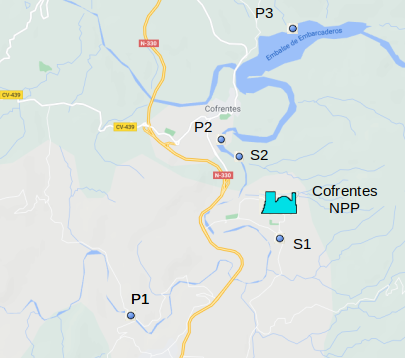
\includegraphics[scale=0.5]{2Introduction/CofrentesMaps.png}
\centering
\caption{Tritium sampling locations around Cofrentes NPP.\label{fig:SamplingLocations}}
\end{figure}

\begin{figure}
\centering
    \begin{subfigure}[b]{0.7\textwidth}
    \centering
    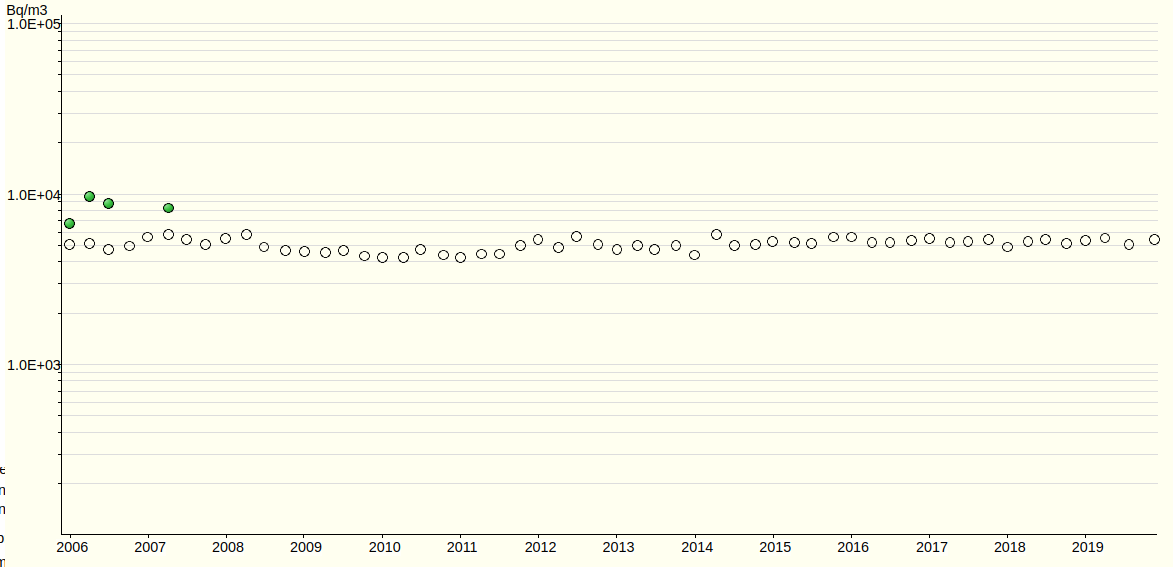
\includegraphics[width=\textwidth]{2Introduction/6km_before.png}  
    \caption{Tritium activity $6~\kilo\meter$ upstream.\label{subfig:TritiumL6kB}}
    \end{subfigure}
    \hfill
    \begin{subfigure}[b]{0.7\textwidth}
    \centering
    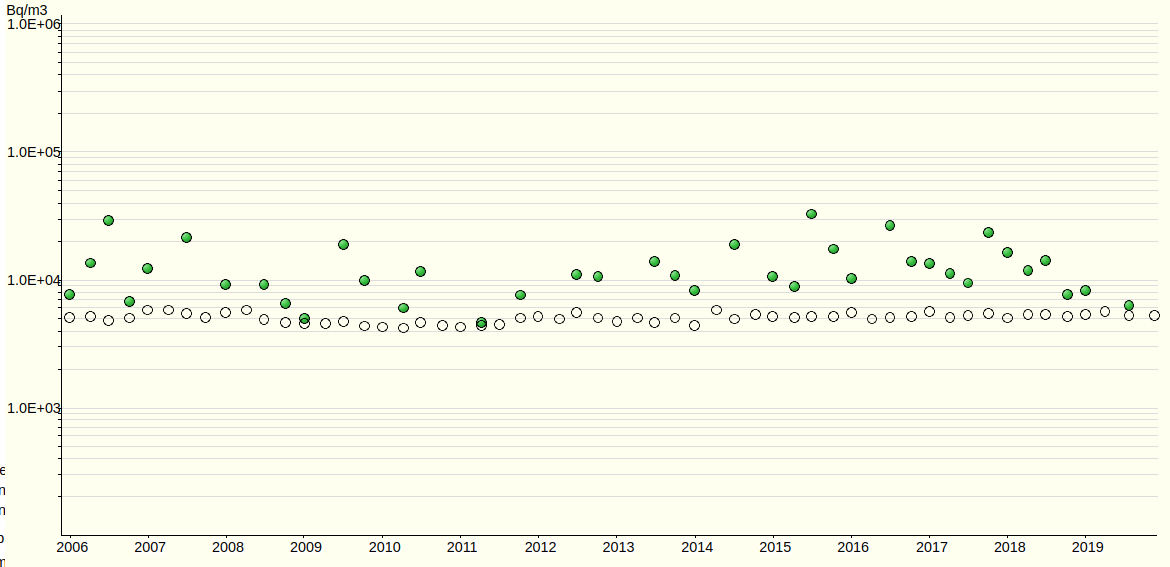
\includegraphics[width=\textwidth]{2Introduction/1km_after.png}  
    \caption{Tritium activity $1~\kilo\meter$ downstream.\label{subfig:TritiumL1kA}}
    \end{subfigure}
    \hfill
    \begin{subfigure}[b]{0.7\textwidth}
    \centering
    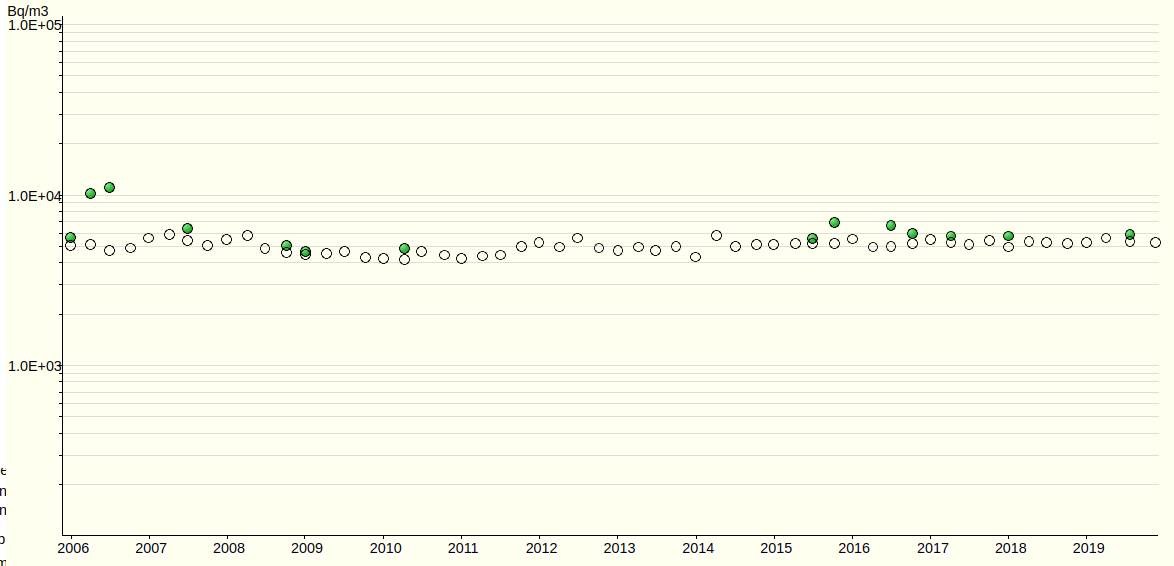
\includegraphics[width=\textwidth]{2Introduction/5km_after.png}  
    \caption{Tritium activity $5~\kilo\meter$ downstream.\label{subfig:TritiumL5kA}}
    \end{subfigure}
 \caption{Tritium activity levels in surface water around Cofrentes NPP from January $2006$ to November $2019$. The white points are used for the detection limit and the green points are used for the measured activity, when it is above the detection limit.~\cite{REM}}
 \label{subfig:MeasurementsCofrentesSurface}
\end{figure}

In these figures, the detection limit and the measured activity are shown using white and green dots, respectively. The measured activity is only displayed when it is larger than the corresponding detection limit. The tritium level in the river increases due to the discharge of the NPP and it is diluted again after $4~\kilo\meter$ downstream, as can be seen from these date. 

Two additional measurements of the tritium level in groundwater have been included, points S1 and S2 on the map in Figure \ref{fig:SamplingLocations}, which are located $1~\kilo\meter$ before and $1~\kilo\meter$ after the NPP. Both tritium levels are shown in the figure \ref{subfig:TritiumLG1kB} and \ref{subfig:TritiumLG1kA} respectively, where it can be observed that they are not affected by the nuclear power plant.

\begin{figure}
\centering
    \begin{subfigure}[b]{0.7\textwidth}
    \centering
    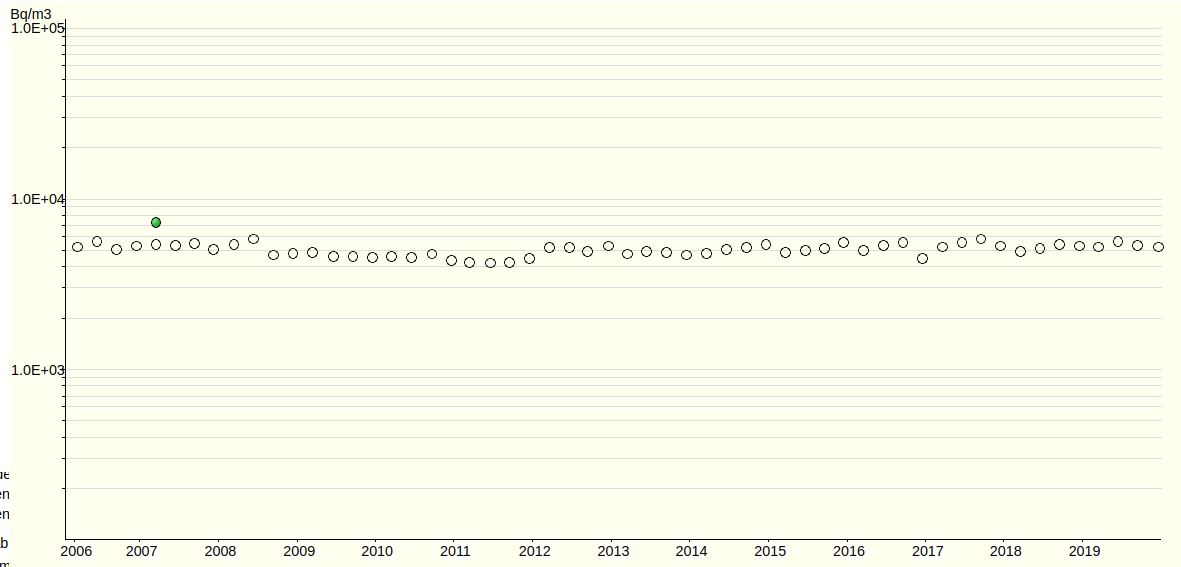
\includegraphics[width=\textwidth]{2Introduction/Subterranea_before.png}  
    \caption{Tritium activity $1~\kilo\meter$ before NPP.\label{subfig:TritiumLG1kB}}
    \end{subfigure}
    \hfill
    \begin{subfigure}[b]{0.7\textwidth}
    \centering
    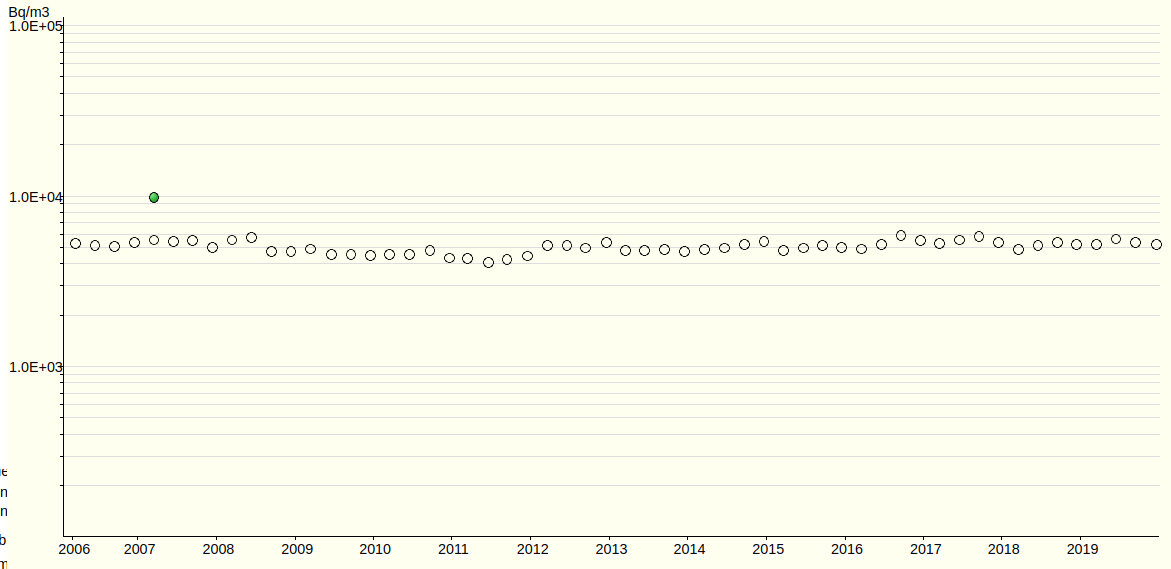
\includegraphics[width=\textwidth]{2Introduction/Subterranea_1_km_later.png}  
    \caption{Tritium activity $1~\kilo\meter$ after NPP.\label{subfig:TritiumLG1kA}}
    \end{subfigure}
 \caption{Tritium activity levels in groundwater around Cofrentes NPP from January $2006$ to November $2019$.~\cite{REM}}
 \label{fig:MeasurementsCofrentesGroundWater}
\end{figure}

It is important to note that, although environmental tritium level is affected by NPP, these levels are below the maximum allowed limit. The maximum level of tritium measured since of January 2, 2006 is around $32~\becquerel/\liter$, below to the maximum allowed limit in Europe, $100~\becquerel/\liter$.

Tritium is a radioactive element with a half-life time of $T_{1/2}= 12.32$ years. It has one proton and two neutrons and decays exclusively through $\beta$ radiation. It decay $100\%$ directly to the ground state of the $\ce{^{3}_{2}He}$ isotope of helium, which is a stable nuclei, thorugh the decay scheme of equation \ref{eq:TritiumDecay}:

\begin{equation}
\ce{^{3}_{1}H} \longrightarrow \ce{^{3}_{2}He}  + \ce{e^-}  + \ce{\overline{\nu}_e}
\label{eq:TritiumDecay}
\end{equation}

In Figure \ref{fig:TritiumDecay} the scheme of tritium energy levels is shown. In this decay it is not possible to detect the neutrino because of its extremely weak interaction with matter ($\sigma \propto 10^{-42} ~ \cm^2$ \cite{CrossSeccionNeutrino}) and, since $\ce{^{3}He}$ has a much larger mass than electrons and neutrinos, by conservation of energy and momentum, the energy that is taken by this daughter nucleus is very small. Therefore, the detection of tritium is through its decay electron. 

\begin{figure}
\centering
    \begin{subfigure}[b]{0.45\textwidth}
    \centering
    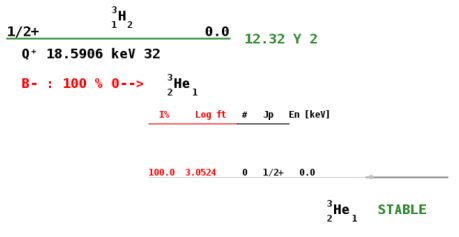
\includegraphics[width=\textwidth]{2Introduction/esquema_niveles_energeticos.png}  
    \caption{Tritium energy levels. \cite{TritiumDecayEnergyLevels}\label{subfig:Energy_levels}}
    \end{subfigure}
    \hfill
    \begin{subfigure}[b]{0.45\textwidth}
    \centering
    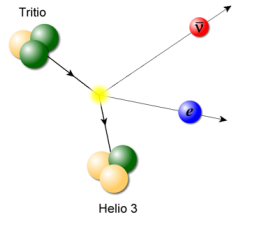
\includegraphics[width=\textwidth]{2Introduction/representacion_desintegracion.png}  
    \caption{Graphic representation of tritium decay \cite{TritiumDecayImage}.\label{subfig:GraphicDesintegration}}
    \end{subfigure}
 \caption{Tritium decay}
 \label{fig:TritiumDecay}
\end{figure}

The energy released in the tritium decay is $Q_\beta=18.6~\keV$, shared between the decay products. Therefore, the energy spectrum of the decay electrons is a continuum with a maximum value of $18,6~\keV$, as shown in Figure \ref{fig:TritiumDecaySpectrum}. This energy spectrum has an average energy of $5.7~\keV$ and the most likely energy is slightly below, around $4.5~\keV$.

\begin{figure}[hbtp]
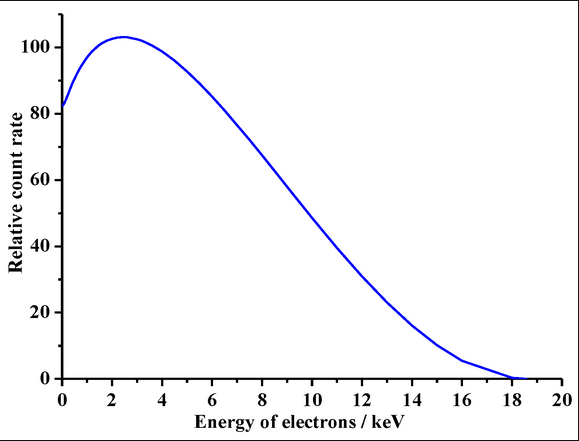
\includegraphics[scale=0.6]{2Introduction/Espectro_tritio.png}
\centering
\caption{Energy spectrum of tritium electrons ~\cite{TritiumEspectrum}\label{fig:TritiumDecaySpectrum}}
\end{figure}

%We have to keep in mind that, although the helium isotope is stable, it will be exited immediately after this decay. As a consequence, after the tritium $\beta^-$ decay, we will have a subsequent dexcitation of the $\ce{^{3}He}$ which will produce photons, $\gamma$, with several well-defined energies that correspond to their energy levels, X-rays\footnote{X-rays are photons whose wavelength are between 0.01 nm and 10 nm. They are produced by nuclear deexitation.}. It will not affect our tritium measurement because, as we will see in Section  \ref{}, the probability of detecting X-rays with the photosensor that will be used is practically negligible.

%Los rayos X son una radiación electromagnética de la misma naturaleza que las ondas de radio, las ondas de microondas, los rayos infrarrojos, la luz visible, los rayos ultravioleta y los rayos gamma. La diferencia fundamental con los rayos gamma es su origen: los rayos gamma son radiaciones de origen nuclear que se producen por la desexcitación de un nucleón de un nivel excitado a otro de menor energía y en la desintegración de isótopos radiactivos, mientras que los rayos X surgen de fenómenos extranucleares, a nivel de la órbita electrónica, fundamentalmente producidos por desaceleración de electrones. La energía de los rayos X en general se encuentra entre la radiación ultravioleta y los rayos gamma producidos naturalmente. Los rayos X son una radiación ionizante porque al interactuar con la materia produce la ionización de los átomos de la misma, es decir, origina partículas con carga (iones). 

The releasing energy of the tritium decay, is very low. In fact, it is the radioactive isotope with the lowest energy released in its $\beta$ disintegration \cite{TritiumHandling}. Consequently, the $\beta$ particle which is emitted in this tritium decay will have a very small mean free path, shown in Table \ref{tab:MeanFreePathTritium}.

\begin{table}[htbp]
\begin{center}
\begin{tabular}{|c|c|c|}
\hline
Material & P. Depth ($5.7~\keV$) & P. Depth ($18.6~\keV$)\\
\hline \hline \hline
$\ce{\ce{^{3}_{1}H_2}}$ & 0.26 cm & 3.2 cm \\ \hline
Air & 0.036 cm & 0.45 cm \\ \hline
\parbox{10em}{\centering Water, soft tissue\\  (solid matter with a \\  density of $1~\gram\cdot\cm^{-3}$)} & 0.42 $\mu\meter$ & 5.2 $\mu\meter$ \\ \hline
\end{tabular}
\caption{Penetration depth for decay electron of mean ($5,7~\keV$) and maximum ($18,6~\keV$) energies in different media (tritium gas and air at standard conditions of temperature ($273~\kelvin$) and preassure ($1$ atm), STP, and water)~\cite{MeanFreePathDocument}}.
\label{tab:MeanFreePathTritium}
\end{center}
\end{table}

This short mean free path is a major issue in tritium detection, as it makes more difficult the electron detection, which will require a highly sensitive detector. It also means that tritium electrons have a low penetration in our body and they are easily stopped with clothes or laboratory gloves, resulting in a low radiological hazard of external tritium. Nevertheless, the danger of tritium increases when it is ingested or inhaled since it can bind anywhere that hydrogen can and perform the same chemical reactions, sometimes with higher rate if the tritium concentration is high enough to catalyze the reaction. 

Tritium can be absorbed in our body in three different ways, gaseous tritium (mainly HT), tritiated water (mainly HTO) and organically bound tritium (called OBT).

\begin{itemize}
\item{} The gaseous tritium, which is normally found mixed in the air, is the least important since less than a $3-5 \cdot{} 10^{-3}~\%$ is absorbed by the human body, which is insignificant \cite{TritiumHandling}. However, it can be transformed into tritiated water, more harmful from a radiobiological point of interest \cite{TritiumHandling}, through the oxidation and exchange reactions by equations \ref{eq:OxidationExchange}:

\begin{equation}
\begin{split}
& Oxidation: \qquad \qquad \qquad \qquad \qquad \qquad Exchange\\
& 2\cdot{}\ce{HT} + \ce{O_2} \rightarrow 2 \cdot{} \ce{HTO} ~ \quad \qquad \qquad \qquad \ce{HT} + \ce{H_2 O} \rightarrow \ce{H_2} + \ce{HTO}\\
& 2\cdot{}\ce{T_2} + \ce{O_2} \rightarrow 2 \cdot{} \ce{T_2 O} \qquad \qquad \qquad \qquad \ce{T_2} + \ce{H_2 O} \rightarrow \ce{HT} + \ce{HTO}
\label{eq:OxidationExchange}
\end{split}
\end{equation}

\item{} Tritiated water, which is normally found in drinking water and food, has a larger impact since the $99\%$ of it is absorbed \cite{TritiumHandling}. Its biological life time corresponds to the water cycle in the body, around $9.5$ days ($\pm50\%$), time during which tritium will remain in our body \cite{TritiumHandling, FranceTritiumEnvironment, EstimationTritiumDosi}. As in water, the biological life time of tritiated water can vary due to various external parameters such as temperature, humidity, drinking habits, etc. or reduced with the use of diuretics \cite{TritiumHandling}.

\item{} Organically bound tritium, normally found in food, generally forms a covalent bond with a carbon and it corresponds to $5-10~\%$ of tritium absorbed in the body. Although it is less absorbed in the body than tritiated water, it can be more dangerous since it has a longer biological life time. The biological life time of this tritium type depends on the affinity of the organic molecule to the different biological tissues and it can vary from tens to hundreds of days (larger than the ICRP estimate) \cite{FranceTritiumEnvironment, EstimationTritiumDosi, EstimationTritiumDosiRats, EstimationTritiumDosiKangarooRats}.
\end{itemize}

There are many studies showing that tritium in living matter can cause the same effects than X-rays or $\gamma$ rays, which are mutations, tumors, cancer, genetic effects, reproductive effects, etc \cite{StraumeTritiumHazard, RytoemaaTritiumHazard}. In fact, the consequences of tritium radiation can be worse than a similar $\gamma$ radiations since its biological efficiency\footnote{The biological efficiency is used to quantify the damage produced in the living cells due to an external radiation.} is two or three times larger \cite{StraumeTritiumHazard}.

In summary, tritium is a naturally occurring radioactive element that can affect health if it is released excessively. Because of that, each country has developed a legislation, shown in section \ref{sec:Legislation}, to manage the release of tritium and ensure that these background levels are safe for health.



%Tritium has different physical properties than other natural isotopes of the hydrogen like different boiling points as shown in Table \ref{tab:BoilingPoints} or the property of self-radiolysis which only happens when radioactive elements are involved. In the case of tritium dissolved in water, it is normally found forming the $\ce{HTO}$ molecule. There, the auto-radiolysis ocurrs because the energy released in tritium decay is larger than the energy bond of oxigen and hydrogen in water molecules ($5.2~\eV$) or the ionization energy of water molecules ($12.6~\eV$) so it can break up these molecules \cite{AutoRadyolisis}. Due to the auto-radiolysis, some radicals appear in the water, increasing its corrosivity. It is a fact that we have to take into account when choosing the materials that will make up the TRITIUM detector.

%\begin{table}[htbp]
%\begin{center}
%\begin{tabular}{|l|l|l|}
%\hline
%Molecule & Boiling point (for gases) ($\kelvin$) & oxidation form\\
%\hline \hline \hline
%$\ce{H_2}$ & 20.39 & $\ce{H_2 O}$ \\ \hline
%$\ce{HD}$ & 22.14 & $\ce{HDO}$ \\ \hline
%$\ce{HT}$ & 22.92 & $\ce{HTO}$ \\ \hline
%$\ce{D_2}$ & 23.66 & $\ce{D_2 O}$ \\ \hline
%$\ce{DT}$ & 24.38 & $\ce{DTO}$ \\ \hline
%$\ce{T_2}$ & 25.04 & $\ce{T_2 O}$ \\ \hline
%\end{tabular}
%\caption{Gas molecules of hydrogen isotopes and their boiling point and oxidation form.~\cite{}}
%\label{tab:BoilingPoints}
%\end{center}
%\end{table}

%Although tritium has different physical properties it has almost the same chemical behaviour than other hydrogen isotopes. Tritium, like hydrogen, is a gas at STP forming a two-atom molecules which can be $\ce{HT}$, $\ce{DT}$ and $\ce{T_2}$. 


%Due to this chemical similarity tritiated water can perform the same chemical processes than non-radiactive water, sometimes with higher rate if the tritium concentration is high enough to catalyze the reaction. Its biological hazard comes from this chemical similarity since tritiated water is able to substitute normal water in human body. 
